% Copyright (C) 2007 Technical University of Liberec.  All rights reserved.
%
% Please make a following reference to Flow123d on your project site if you use the program for any purpose,
% especially for academic research:
% Flow123d, Research Centre: Advanced Remedial Technologies, Technical University of Liberec, Czech Republic
%
% This program is free software; you can redistribute it and/or modify it under the terms
% of the GNU General Public License version 3 as published by the Free Software Foundation.
%
% This program is distributed in the hope that it will be useful, but WITHOUT ANY WARRANTY;
% without even the implied warranty of MERCHANTABILITY or FITNESS FOR A PARTICULAR PURPOSE.
% See the GNU General Public License for more details.
%
% You should have received a copy of the GNU General Public License along with this program; if not,
% write to the Free Software Foundation, Inc., 59 Temple Place - Suite 330, Boston, MA 021110-1307, USA.
%


\section{Meshes of Mixed Dimension}
Unique feature common to all models in Flow123d is the support of
domains with mixed dimension. 
Let $\Omega_{3} \subset \Real^3$ be an open set representing continuous approximation of porous and fractured medium.
Similarly, we consider a~set of 2D manifolds $\Omega_2\subset\overline\Omega_3$, representing the 2D fractures and a~set of 1D manifolds $\Omega_1\subset \overline\Omega_2$ 
representing the 1D channels or preferential paths (see Fig \ref{fig:multi-dim}).
We assume that $\Omega_2$ and $\Omega_1$ are polytopic (i.e. polygonal and piecewise linear, respectively).
For every dimension $d=1,2,3$, we introduce a~triangulation $\mathcal{T}_{d}$ of the open set $\Omega_d$
that consists of finite elements $T_{d}^{i},$\ $i = 1,\dots,N_{E}^{d}$.
The elements are simplices, i.e. lines, triangles and tetrahedra, respectively.

\begin{figure}[h]
\centering
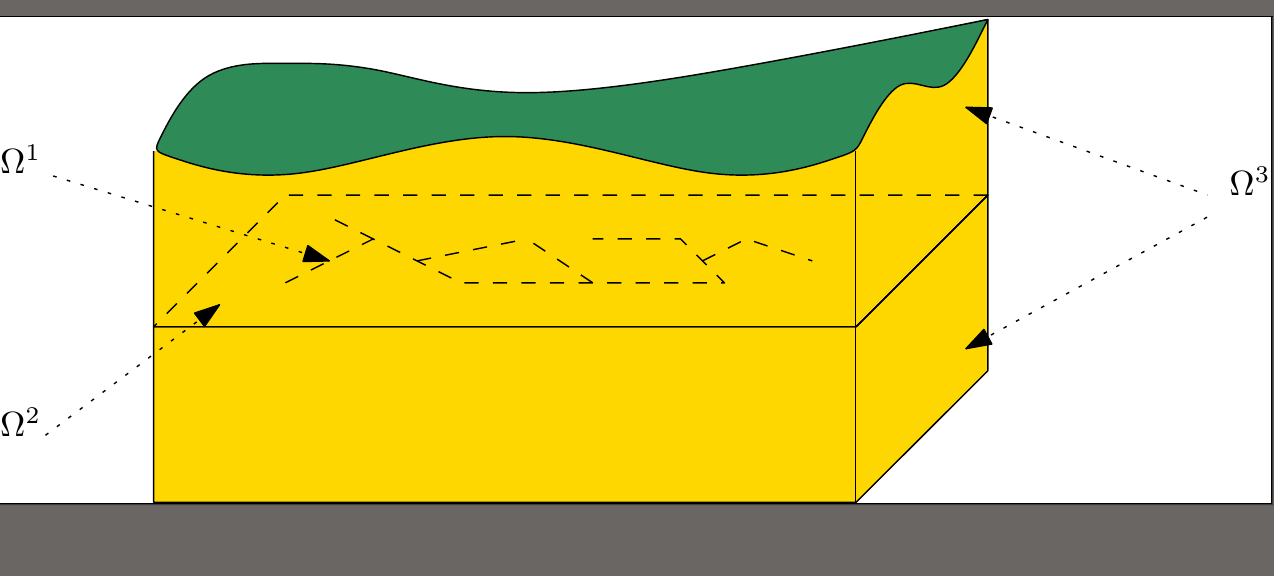
\includegraphics[width=10cm]{\fig/ground_fractures}
\caption{
    \label{fig:multi-dim}
    Scheme of a~problem with domains of multiple dimensions.
}
\end{figure}

Present numerical methods used by the software require meshes satisfying the compatibility conditions
\begin{equation}
        T_{d-1}^i \cap T_d \subset \mathcal{F}_d,   \qquad \text{where } \mathcal{F}_d = \bigcup_{k} \partial T_{d}^{k}
\end{equation}
and
\begin{equation}
        T_{d-1}^i \cap \mathcal{F}_d    \text{ is either $T_{d-1}^i$ or $\emptyset$}    
\end{equation}
for every $i\in\{1,\dots, N_{E}^{d-1}\}$, $j\in\{1,\dots,N_{E}^{d}\}$,  and $d=2,3$. 
That is, the $(d-1)$-dimensional elements are either between $d$-dimensional elements and
match their sides or they poke out of $\Omega_d$. Support for a~coupling between non-compatible
meshes of different dimensions is under development and partially supported by the Darcy Flow model.

\section{Advection-Diffusion Processes on Fractures}
\label{sc:ad_on_fractures}
This section presents derivation of an abstract advection-diffusion process on 2D and 1D manifolds and its coupling with
the higher dimensional domains. The reader not interested in the details of this approximation may skip directly to
the later sections describing mathematical models of individual physical processes.

As was already mentioned, the unique feature of Flow123d is support of models living on 2D and 1D manifolds. The aim is to capture 
features significantly influencing the solution despite of their small cross-section. Such a~tiny features are
challenging for numerical simulations since a~direct discretization requires highly refined
computational mesh. One possible solution is to model these features (fractures, channels) 
as lower dimensional objects (2D and 1D manifolds) and introduce their coupling with the surrounding continuum.
The equations modeling a~physical process on a~manifold as well as its coupling to the model in the surrounding continuum
has to be derived from the model on the 3D continuum. This section presents such a~procedure for the case of the abstract
advection-diffusion process inspired by the paper \cite{martin_modeling_2005}. Later, we apply this abstract approach to 
particular advection-diffusion processes: Darcy flow, solute transport, and heat transfer.

Let us consider a~fracture as a~strip domain 
\[
 \Omega_f \subset [0,\delta] \times \Real^{d-1}
\]
for $d=2$ or $d=3$ and surrounding continuum domains
\[
 \Omega_1 \subset (-\infty,0)\times \Real^{d-1},
 \Omega_2 \subset (\delta,\infty)\times \Real^{d-1}.
\]
Further, we denote by $\gamma_i$, $i=1,2$ the fracture faces common with domains $\Omega_1$ and $\Omega_2$ respectively.
By $x$, $\vc y$ we denote normal and tangential coordinate of a~point in $\Omega_f$. 
We consider the normal vector  $\vc n=\vc n_1=-\vc n_2=(1,0,0)^\top$.
An advection-diffusion process is given by equations:
\begin{align}
  \label{eq:fr:continuity}
  \prtl_t w_i + \div \vc j_i &= f_i&&  \text{on } \Omega_i,\ i=1,2,f,\\
  \label{eq:fr:flux}
  \vc j_i &= - \tn A_i\grad u_i + \vc b_i w_i&& \text{on } \Omega_i,\ i=1,2,f,\\
  \label{eq:fr:Dirichlet}
  u_i &= u_f&& \text{on } \gamma_i,\ i=1,2,\\
  \label{eq:fr:Neumann}
  \vc j_i \cdot \vc n &= \vc j_f \cdot \vc n&& \text{on } \gamma_i,\ i=1,2,
\end{align}
where $w_i=w_i(u_i)$ is the conservative quantity and $u_i$ is the principal unknown, $\vc j_i$ is the flux of $w_i$, $f_i$ is the source term,
$\tn A_i$ is the diffusivity tensor and $\vc b_i$ is the velocity field. We assume that the tensor $\tn A_f$ is symmetric positive definite 
with one eigenvector in the direction $\vc n$. Consequently the tensor has the form:
\[
 A_f = \begin{pmatrix} 
            a_n & 0  \\
            0 & \tn A_t
       \end{pmatrix}
\]
Furthermore, we assume that $\tn A_f(x, \vc y)=\tn A_f(\vc y)$ is constant in the normal direction.

Our next aim is to integrate equations on the fracture $\Omega_f$ in the normal direction 
and obtain their approximations on the surface $\gamma=\Omega_f \cap \{x=\delta/2\}$ running through the middle of the fracture. 
For the sake of clarity, we will not write subscript $f$ for quantities on the fracture. 
To make the following procedure mathematically correct we have to assume that functions
$\prtl_x w$, $\prtl_x \grad_{\vc y} u$, $\prtl_x \vc b_{\vc y}$ are continuous and bounded on $\Omega_f$. Here and later on 
$\vc b_x=(\vc b \cdot \vc n)\, \vc n$ is the normal part of the velocity field and $\vc b_{\vc y} = \vc b - \vc b_x$ is the tangential part.
The same notation will be used for normal and tangential part of the field $\vc q$.

We integrate \eqref{eq:fr:continuity} over the fracture opening $[0,\delta]$ and use approximations to get
\begin{equation}
    \label{eq:fracture_continuity}
   \prtl_t (\delta W) - \vc j_2 \cdot \vc n_2 - \vc j_1 \cdot \vc n_1 + \div \vc J = \delta F,
\end{equation}
where for the first term, we have used mean value theorem, first order Taylor expansion, 
and boundedness of $\prtl_x w$ to obtain approximation:
\[
    \int_0^\delta w(x,\vc y) \d x=\delta w(\xi_{\vc y}, \vc y) = \delta W(\vc y) + O(\delta^2\abs{\prtl_x w}),
\]
where
\[
    W(\vc y)=w(\delta / 2,\vc y)=w(u(\delta/2,\vc y))=w(U(\vc y)).
\]
Next two terms in \eqref{eq:fracture_continuity} come from the exact integration 
of the divergence of the normal flux $\vc j_x$.
Integration of the divergence of the tangential flux $\vc j_{\vc y}$ gives the fourth term, where we introduced
\[
\vc J(\vc y) = \int_0^\delta \vc j_{\vc y}(x, \vc y) \d x.
\]
In fact, this flux on $\gamma$ is scalar for the case $d=2$. Finally, we integrate the right-hand side to get 
\[
    \int_0^\delta f(x,\vc y) \d x = \delta F(\vc y) + O(\delta^2\abs{\prtl_x f}),\quad F(\vc y)=f(\delta/2,\vc y). 
\]


Due to the particular form of the tensor $\tn A_f$, we can separately integrate tangential and normal
part of the flux given by \eqref{eq:fr:flux}. Integrating the tangential part and using approximations
\[
    \int_0^\delta  \grad_{\vc y} u(x, \vc y) \d x = \delta \grad_{\vc y} u (\xi_{\vc y}, \vc y) 
    = \delta \grad_{\vc y} U( \vc y) + O\big( \delta^2 \abs{\prtl_x\grad_{\vc y} u} \big) 
\]
and
\[
 \int_0^\delta \big(\vc b_{\vc y} w\big)(x, \vc y) \d x 
  = \delta \vc B(\vc y) W(\vc y) + O\big(\delta^2 \abs{\prtl_x(\vc b_{\vc y} w)} \big)
\]
where
\[
  \vc B(\vc y) = \vc b_{\vc y}(\delta/2, \vc y),
\]
we obtain
\begin{equation}
    \label{eq:fracture_darcy}
   \vc J = -\tn A_t \delta \grad_{\vc y} U + \delta \vc B W + O\big(\delta^2(\abs{\prtl_x\grad_{\vc y} u}+\abs{\prtl_x(\vc b_{\vc y} w)})\big).
\end{equation}


So far, we have derived equations for the state quantities $U$ and $\vc J$ on the fracture manifold $\gamma$. In order to
get a~well-posed problem, we have to prescribe two conditions for boundaries $\gamma_i$, $i=1,2$. To this end, we
perform integration of the normal flux $\vc j_x$, given by \eqref{eq:fr:flux}, separately for the left and right half of the fracture.
Similarly as before we use approximations
\[
 \int_0^{\delta/2} \vc j_x \d x = (\vc j_1 \cdot \vc n_1)\frac{\delta}{2} + O(\delta^2 \abs{\prtl_x \vc j_x})
\]
and 
\[
 \int_0^{\delta/2} \vc b_x w \d x = (\vc b_1 \cdot \vc n_1)\tilde{w}_1\frac{\delta}{2} + O(\delta^2 \abs{\prtl_x \vc b_x}\abs{w} + \delta^2\abs{\vc b_x}\abs{\prtl_x w})
\]
and their counter parts on the interval $(\delta/2, \delta)$ to get
\begin{align}
    \label{eq:fracture_normal_1}
     \vc j_1 \cdot \vc n_1 &= -\frac{2a_n}{\delta} (U - u_1) + \vc b_1\cdot \vc n_1 \tilde{w}_1\\
    \label{eq:fracture_normal_2}
    \vc j_2 \cdot \vc n_2 &= -\frac{2a_n}{\delta} (U - u_2) + \vc b_2\cdot \vc n_2 \tilde{w}_2
\end{align}
where $\tilde w_i$ can be any convex combination of $w_i$ and $W$. Equations \eqref{eq:fracture_normal_1}  
and \eqref{eq:fracture_normal_2} have meaning of a~semi-discretized flux from domains $\Omega_i$ into fracture.
In order to get a~stable numerical scheme, we introduce a~kind of upwind already on this level using a~different convex 
combination for each flow direction:
\begin{align}
   \notag 
   \vc j_i \cdot \vc n_i
       = &-\sigma_i (U - u_i)      \\ 
   \notag
      &+ \big[\vc b_i\cdot \vc n_i\big]^{+} \big(\xi w_i + (1-\xi) W\big)       \\
      \label{eq:fracture_normal}
      &+ \big[\vc b_i\cdot \vc n_i\big]^{-} \big((1-\xi) w_i + \xi W\big), \qquad i=1,2
\end{align}
where $\sigma_i = \frac{2a_n}{\delta}$ is the transition coefficient and the parameter $\xi\in [\frac12, 1]$ can be used to interpolate
between upwind ($\xi = 1$) and central difference ($\xi=\frac12$) scheme. Equations \eqref{eq:fracture_continuity}, \eqref{eq:fracture_darcy}, and
\eqref{eq:fracture_normal} describe the general form of the advection-diffusion process on the fracture and its communication with 
the surrounding continuum which we shall later apply to individual processes.
